\section{Orientierte Winkel modulo \texorpdfstring{$\boldsymbol{180^\circ}$}{180°}}\label{kapitel:OrientierteWinkel}
Lagebeziehungsfallunterscheidungen sind lästig, rauben wertvolle Zeit beim Aufschreiben und führen zu unnötigen Punktabzügen, wenn ihr sie nicht ordentlich macht. In diesem Kapitel lernt ihr eine Technik kennen, mit der ihr euch diesen Ärger sparen könnt.

Wir beginnen mit einigen allgemeinen Betrachtungen. Seien $g$ und $h$ zwei Geraden, die sich in einem Punkt $S$ schneiden. Sei $K_{g,h}$ die Menge aller Winkel $\varphi$, sodass eine Drehung mit Zentrum $S$ und Winkel $\varphi$ die Gerade $g$ auf die Gerade $h$ abbildet. Wenn $\varphi_0$ in der Menge $K_{g,h}$ liegt, dann sind $\varphi_0 + 180^\circ,\varphi_0 + 360^\circ,\varphi_0 + 540^\circ,\dotsc$ offensichtlich ebenfalls Elemente von $K_{g,h}$. Das gleiche gilt für $\varphi_0 - 180^\circ,\varphi_0 - 360^\circ,\dotsc$. Umgekehrt muss aber auch jeder Winkel $\varphi\in K_{g,h}$ von der Form $\varphi=\varphi_0 + k\cdot 180^\circ$ für ein $k\in \mathbb Z$ sein. Denn wenn sowohl eine Drehung um $\varphi_0$ als auch eine Drehung um $\varphi$ die Gerade $g$ auf $h$ abbildet, dann muss eine Drehung um $\varphi - \varphi_0$ die Gerade $g$ auf sich selber abbilden, also muss $\varphi - \varphi_0$ ein ganzzahliges Vielfaches von $180^\circ$ sein. Wir erhalten folglich
\begin{equation*}
	K_{g,h}=\braces*{\varphi_0 + k\cdot 180^\circ\ \middle|\  k\in \mathbb Z}\,.
\end{equation*}
Mit anderen Worten, $K_{g,h}$ ist eine \emph{Restklasse modulo $180^\circ$}. Das soll Folgendes heißen: Genau wie für ganze Zahlen schreiben wir $\alpha\equiv\beta \mod 180^\circ$ für zwei Winkel $\alpha$ und $\beta$, wenn $\alpha - \beta$ ein ganzzahliges Vielfaches von $180^\circ$ ist. In diesem Sinne ist dann
\begin{equation*}
	K_{g,h}=\braces*{\varphi\ \middle|\ \varphi\equiv\varphi_0 \mod 180^\circ}\,,
\end{equation*}
wofür die Bezeichnung \emph{Restklasse modulo $180^\circ$} allemal gerechtfertigt ist.
\begin{definition}
	Mit $\winkel(g,h)$ bezeichnen wir einen beliebigen Repräsentanten $\varphi_0\in K_{g,h}$ der Restklasse $K_{g,h}$. Falls $g$ und $h$ parallele Geraden sind, definieren wir $\winkel(g,h)\coloneqq 0^\circ$.
\end{definition}

Genau wie bei ganzen Zahlen könnt ihr euch überlegen, dass Addition und Subtraktion von Winkeln sowie Multiplikation mit ganzen Zahlen auch modulo $180^\circ$ funktionieren. Solange wir also nur modulo $180^\circ$ rechnen, kommt es nicht darauf an, welchen konkreten Repräsentanten wir für $\winkel (g,h)$ gewählt haben.

Der Vorteil von orientierten Winkeln modulo $180^\circ$ liegt darin, dass sie sich unter Addition so verhalten, wie wir es intuitiv erwarten würden.
\begin{satzmitnamen}[Eigenschaften von orientierten Winkeln modulo $\boldsymbol{180^\circ}$]
	Sei $n\geqslant 2$ und seien $g_1,\dotsc,g_n$ Geraden in der Ebene.
	\begin{enumerate}
		\item Es gilt $\winkel(g_1,g_2) + \winkel(g_2,g_3)+ \dotsb + \winkel(g_{n-1},g_n) \equiv \winkel(g_1,g_n) \mod 180^\circ$.\label{eigenschaft:OrientierteWinkelAdditiv}
		\item Es gilt $\winkel(g_1,g_2) + \winkel(g_2,g_3) + \dotsb + \winkel(g_n,g_1) \equiv 0^\circ  \mod 180^\circ$.\label{eigenschaft:OrientierteWinkelAddierenZuNull}
		\item Wenn $g$ und $h$ beliebige Geraden sind, dann ist $\winkel(g,h) \equiv -\winkel(h,g) \mod 180^\circ$.\label{eigenschaft:OrientierungVorzeichen}
	\end{enumerate}
\end{satzmitnamen}
\begin{proof}
	Wir beweisen zunächst Eigenschaft~\ref{eigenschaft:OrientierteWinkelAddierenZuNull}. Dafür benutzen wir folgenden Fakt: Wenn $\sigma$ und $\tau$ zwei Drehungen oder Verschiebungen sind, dann ist ihre Hintereinanderausführung $\sigma\circ\tau$ wieder eine Drehung oder Verschiebung (das gilt insbesondere auch dann, wenn $\sigma$ und $\tau$ zwei Drehungen sind, die \emph{nicht} das gleiche Zentrum haben). Wenn ihr diesen Fakt noch nicht kanntet, könnt ihr ihn im Kapitel \emph{\embrace{Dreh-}Streckungen} im Heft für die Klasse~10 nachlesen.
	
	Für $i=1,2,\dotsc,n$ sei $\sigma_i$ eine Drehung um den Schnittpunkt von $g_i$ und $g_{i+1}$, die $g_i$ auf $g_{i+1}$ abbildet (dabei setzen wir $g_{n+1}\coloneqq g_1$). Nach Definition ist der Drehwinkel von $\sigma_i$ genau $\winkel (g_i,g_{i+1})$. Falls $g_i$ und $g_{i+1}$ parallel sind, definieren wir $\sigma_i$ stattdessen als eine Verschiebung, die $g_i$ auf $g_{i+1}$ abbildet. Auch in diesem Fall ist der \glqq Drehwinkel\grqq\ von $\sigma$ genau $\winkel (g_i,g_{i+1})=0^\circ$. Nach obigem Fakt ist die Hintereinanderausführung $\sigma\coloneqq \sigma_n\circ\sigma_{n-1}\circ\dotsb\circ\sigma_1$ wieder eine Drehung oder eine Verschiebung. Da sich Drehwinkel bei Hintereinanderausführung addieren, ist der Drehwinkel von $\sigma$ durch $\winkel(g_1,g_2) + \winkel(g_2,g_3) + \dotsb + \winkel(g_n,g_1)$ gegeben. Andererseits bildet $\sigma$ die Gerade $g_1$ auf sich selbst ab. Der Drehwinkel muss also $\equiv 0^\circ\mod 180^\circ$ sein. Genau das wollten wir zeigen.
	
	Nachdem Eigenschaft~\ref{eigenschaft:OrientierteWinkelAddierenZuNull} nun bewiesen ist, folgt Eigenschaft~\ref{eigenschaft:OrientierungVorzeichen} sofort als der Spezialfall $n=2$. Schließlich folgt Eigenschaft~\ref{eigenschaft:OrientierteWinkelAdditiv} aus einer Kombination von~\ref{eigenschaft:OrientierteWinkelAddierenZuNull} und~\ref{eigenschaft:OrientierungVorzeichen}.
\end{proof}

Bisher haben wir nur über Winkel zwischen Geraden geredet und nicht über solche, die von zwei Punkten $A$ und $B$ sowie einem Scheitelpunkt $S$ aufgespannt werden. Als Ersatz für den Winkel $\winkel ASB$ werden wir immer den orientierten Winkel $\winkel(AS,BS)$ modulo $180^\circ$ verwenden.

Die meisten Sätze über Winkel lassen sich zu Sätzen über orientierte Winkel modulo $180^\circ$ umformulieren. Üblicherweise wird die Aussage dabei eleganter. Zum Beispiel lassen sich der Peripheriewinkelsatz und der Satz über die gegenüberliegenden Winkel im Sehnenviereck zu folgendem Satz vereinigen -- eleganter geht es nicht:
\begin{satzmitnamen}[Orientierter Peripheriewinkelsatz]
	Vier Punkte $A$, $B$, $C$ und $D$ liegen genau dann auf einem Kreis, wenn Folgendes gilt:
	\begin{equation*}
		\winkel(AC,BC)\equiv\winkel(AD,BD) \mod 180^\circ\,.
	\end{equation*}
\end{satzmitnamen}
Wenn ihr in einer Aufgabe zeigen sollt, dass vier Punkte auf einem Kreis liegen, könnt ihr wie gewohnt eine Winkeljagd durchführen, ohne euch zunächst darüber Gedanken zu machen, ob es noch andere Lagebeziehungen als in eurer Skizze geben könnte. Beim Aufschreiben übersetzt ihr dann eure Argumente in orientierte Winkel modulo $180^\circ$ und formuliert alle Umformungen mithilfe der obigen Eigenschaften. Mit etwas Übung dauert das kaum länger als normalerweise. Dadurch habt ihr alle anderen Lagefälle automatisch mit abgedeckt, ihr spart euch jede Menge Zeit und ihr bekommt keine ärgerlichen Punktabzüge.


Ebenso elegant lässt sich der Sehnen-Tangentenwinkelsatz formulieren:
\begin{satzmitnamen}[Orientierter Sehnen-Tangentenwinkelsatz]
	Sei $ABC$ ein Dreieck. Eine Gerade $t$ durch $B$ ist genau dann Tangente an den Umkreis $\odot ABC$, wenn Folgendes gilt:
	\begin{equation*}
		\winkel(AC,BC)\equiv\winkel(AB,t) \mod 180^\circ\,.
	\end{equation*}
\end{satzmitnamen}
Beim Zentri-Peripheriewinkelsatz müssen wir ein wenig aufpassen:
\begin{satzmitnamen}[Orientierter Zentri-Peripheriewinkelsatz]\label{prop:ZPWS}
	Sei $\Omega$ ein Kreis mit Mittelpunkt $O$ und $A$, $B$ zwei gegebene Punkte auf $\Omega$.
	\begin{enumerate}
		\item Sei $M$ der Mittelpunkt von $\overline{AB}$. Dann liegt ein dritter Punkt $C$ genau dann auf $\Omega$, wenn
		\begin{equation*}
			\winkel(AC,BC)\equiv \winkel(AO,MO)\mod 180^\circ\,.
		\end{equation*}
		\item Wenn $C$ auf $\Omega$ liegt, dann gilt
		\begin{equation*}
			2\winkel(AC,BC)\equiv \winkel(AO,BO)\mod 180^\circ\,.
		\end{equation*}
	\end{enumerate}
\end{satzmitnamen}
\begin{itemize}
	\item[\Warnung] Beachte, dass die zweite Aussage im orientierten Zentri-Peripheriewinkelsatz \emph{keine} \glqq genau dann, wenn\grqq-Aussage ist: Die Bedingung $2\winkel(AC,BC)\equiv \winkel(AO,BO)\mod 180^\circ$ reicht noch nicht aus, um zu schließen, dass $C$ auf dem Kreis $\Omega$ um $O$ durch $A$ und $B$ liegt. Wenn wir nämlich $\alpha$ fixieren, wird die Gleichung $2\winkel(AC,BC)\equiv \alpha\mod180^\circ$ sowohl von $\winkel ACB=\alpha/2$, als auch von $\winkel ACB=90^\circ+\alpha/2$ gelöst, aber nur einer von beiden Fällen sorgt auch dafür, dass $C$ auf $\Omega$ liegt.
	
	Allgemein lassen sich orientierte Winkel modulo $180^\circ$ \emph{nicht} durch ganze Zahlen teilen. Zum Beispiel haben wir gerade gesehen, dass der Ausdruck \glqq$\alpha/2$\grqq\ modulo $180^\circ$ gar nicht wohldefiniert ist. Praktisch hat das aber so gut wie keine Auswirkungen, solange ihr eure Lösungen geschickt formuliert.
	\item[\Warnung] Orientierte Winkel modulo $180^\circ$ können wir auch nicht einfach so in Sinus und Cosinus einsetzen; zum Beispiel ist ja $\sin(\alpha + 180^\circ)=-\sin(\alpha)$, obwohl $\alpha + 180^\circ\equiv \alpha\mod180^\circ$ gilt. Andererseits ist das Vorzeichen aber auch das einzige Problem. Die Ausdrücke $\abs{\sin (\alpha)}$ und $\abs{\cos(\alpha)}$ sind also immer noch wohldefiniert, auch wenn $\alpha$ nur modulo $180^\circ$ bestimmt ist. Zudem haben Tangens und Cotangens die Periode $180^\circ$. Hier kommen wir also überhaupt nicht in Schwierigkeiten.
\end{itemize}
Mit orientierten Winkeln modulo $180^\circ$ lässt sich ein denkbar einfaches Kriterium formulieren, wann sich drei Kreise in einem Punkt schneiden. %Der bekannte \emph{Satz von Miquel} und seine Varianten sind einfache Folgerungen.
\begin{satzmitnamen}[Lemma]
	Gegeben seien sechs Punkte $A$, $B$, $C$ und $A'$, $B'$, $C'$. Dann schneiden sich sie Umkreise $\odot ABC'$, $\odot BCA'$, $\odot CAB'$ genau dann in einem Punkt, wenn die folgende Bedingung gilt:
	\begin{equation*}
		\winkel(AC',BC') + \winkel (BA',CA') + \winkel(CB', AB')\equiv 0 \mod 180^\circ\,.
	\end{equation*}
\end{satzmitnamen}

\begin{proof}
	Sei $T$ der von $B$ verschiedene Schnittpunkt der Umkreise $\odot ABC'$ und $\odot BCA'$. Nach dem orientierten Peripheriewinkelsatz liegt $T$ genau dann auf $\odot CAB'$, wenn die Kongruenz $\winkel(CT,AT)\equiv\winkel (CB',AB') \mod 180^\circ$ gilt. Nun ist aber
	\begin{alignat*}{2}
		0^\circ&\equiv \winkel(CT,AT) +\winkel(AT,BT) + \winkel(BT,CT) &&\mod 180^\circ\\
		&\equiv \winkel(CT,AT) + \winkel(AC',BC') + \winkel(BA',CA') &&\mod 180^\circ\,,
	\end{alignat*}
	wobei wir Eigenschaft~\ref{eigenschaft:OrientierteWinkelAddierenZuNull} sowie den orientierten Peripheriewinkelsatz für die Umkreise $\odot ABC'$ und $\odot BCA'$ verwendet haben. Die Behauptung folgt sofort.
\end{proof}
\begin{figure}[ht]
	\centering
	\begin{tabularx}{\textwidth}{X c X c X}
		& 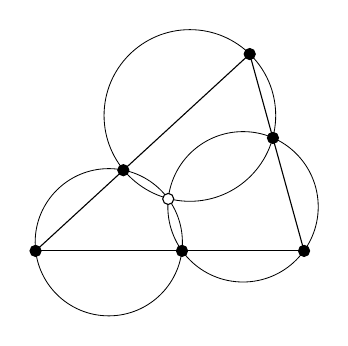
\begin{tikzpicture}[x=0.5cm,y=0.5cm]
			\clip (-1.96,-3.7) rectangle (5.47,3.67);
			\draw (3.68,3)-- (-1.76,-2);
			\draw (-1.76,-2)-- (5.06,-2);
			\draw (3.68,3)-- (5.06,-2);
			\draw [line width=0.3] (0.1,-1.78) circle (1.87);
			\draw [line width=0.3] (3.51,-0.88) circle (1.91);
			\draw [line width=0.3] (2.16,1.44) circle (2.18);
			\draw [fill=black] (3.68,3) circle (2pt);
			\draw [fill=black] (-1.76,-2) circle (2pt);
			\draw [fill=black] (5.06,-2) circle (2pt);
			\draw [fill=black] (0.47,0.05) circle (2pt);
			\draw [fill=black] (1.96,-2) circle (2pt);
			\draw [fill=black] (4.27,0.87) circle (2pt);
			\draw [fill=white] (1.61,-0.68) circle (2pt);
		\end{tikzpicture} & & 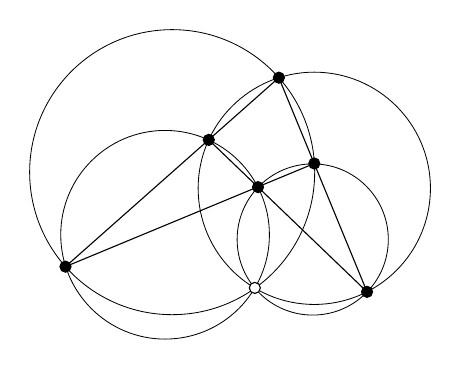
\begin{tikzpicture}[x=0.5cm,y=0.5cm]
			\clip (-1.74,-3.55) rectangle (8.54,4.41);
			\draw  (-0.78,-1.66)-- (4.64,3.14);
			\draw  (4.64,3.14)-- (6.88,-2.3);
			\draw  (6.88,-2.3)-- (2.86,1.56);
			\draw  (-0.78,-1.66)-- (5.54,0.96);
			\draw [line width=0.3] (1.75,-0.85) circle (2.65);
			\draw [line width=0.3] (5.5,-0.97) circle (1.92);
			\draw [line width=0.3] (1.93,0.74) circle (3.62);
			\draw [line width=0.3] (5.54,0.33) circle (2.95);
			\draw [fill=black] (-0.78,-1.66) circle (2pt);
			\draw [fill=black] (4.64,3.14) circle (2pt);
			\draw [fill=black] (6.88,-2.3) circle (2pt);
			\draw [fill=black] (2.86,1.56) circle (2pt);
			\draw [fill=black] (5.54,0.96) circle (2pt);
			\draw [fill=black] (4.11,0.36) circle (2pt);
			\draw [fill=white] (4.03,-2.20) circle (2pt);
		\end{tikzpicture} & \\
		& Satz von Miquel & & Vier-Geraden-vier-Kreise-Satz & 
	\end{tabularx}
\end{figure}

Als direkte Folgerungen erhalten wir den bekannten \emph{Satz von Miquel} und den Vier-Geraden-vier-Kreise-Satz, die wir hier beide illustriert haben. (\emph{Übungsaufgabe: Trage die Punkte $A$, $B$, $C$ und $A'$, $B'$, $C'$ in die Skizzen ein, sodass ersichtlich wird, dass Spezialfälle des Lemmas vorliegen.})



Zuletzt wollen wir an einem Beispiel vorführen, wie eine Lösung mit orientierten Winkeln modulo $180^\circ$ aussehen kann. Die betreffende Aufgabe ist an sich nicht sonderlich schwierig und ihr werdet sie bestimmt schnell herausbekommen. Dennoch haben die meisten Teilnehmenden der damaligen Klausur höchsten 8 oder 9 von 10 Punkten bekommen, weil außerordentlich viele Lagefälle auftreten können.
\begin{aufgabe*}
	Zwei Kreise $\omega_1$ und $\omega_2$ mit den Mittelpunkten $O_1$ bzw.\ $O_2$ schneiden sich in den beiden verschiedenen Punkten $A$ und $B$. Eine durch $A$ verlaufende Gerade schneide $\omega_1$ erneut im Punkt $C\neq A$ und $\omega_2$ in $D\neq A$. Die Geraden $CO_1$ und $DO_2$ schneiden sich in $X$. Beweise, dass die vier Punkte $O_1$, $O_2$, $B$ und $X$ auf einem gemeinsamen Kreis liegen.
\end{aufgabe*}
\begin{figure}[ht]
	\centering		
	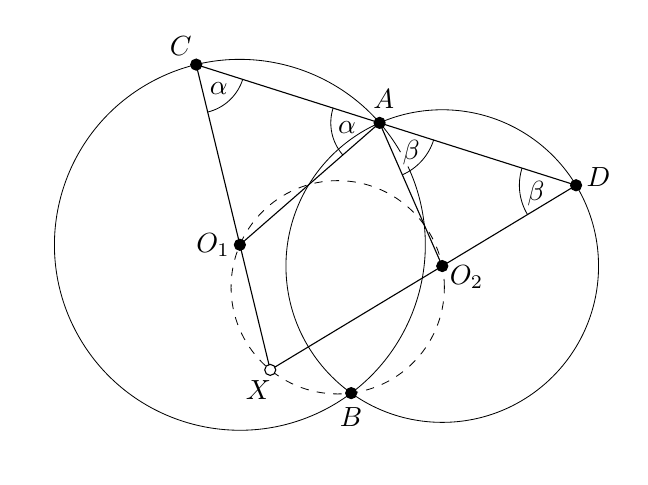
\begin{tikzpicture}[x=0.5cm,y=0.5cm]
		%\clip (-3.42,-5.86) rectangle (10.83,4.3);
		\draw [line width=0.3,shift={(1.34,-1.1)}] (30:4.71) arc (30:385:4.71);
		\draw [line width=0.3] (6.48,-1.64) coordinate (O2) circle (3.97);
		\draw [dashed,line width=0.3] (3.825,-2.179) circle (2.709);
		\coordinate (O1) at (1.34,-1.1);
		\coordinate (A) at (4.889,1.997);
		\coordinate (B) at (4.167,-4.867);
		\coordinate (C) at (0.23,3.477);
		\coordinate (D) at (9.879,0.412);
		\coordinate (X) at (2.111,-4.277);
		\draw (C) to (D) to (X) to cycle;
		\draw (O1) to (A) to (O2);
		\draw [fill=black] (O1) circle (2pt) node[shift={(180:2.25ex)}] {$O_1$};
		\draw [fill=black] (O2) circle (2pt) node[shift={(-25:2.25ex)}] {$O_2$};
		\draw [fill=black] (A) circle (2pt) node[shift={(80:2ex)}] {$A$};
		\draw [fill=black] (B) circle (2pt) node[shift={(270:2ex)}] {$B$};
		\draw [fill=black] (C) circle (2pt) node[shift={(130:2ex)}] {$C$};
		\draw [fill=black] (D) circle (2pt) node[shift={(20:2ex)}] {$D$};
		\draw [fill=white] (X) circle (2pt) node[shift={(240:2ex)}] {$X$};
		\draw [line width=0.3,shift={(C)}] (283.636:0.62cm) arc (283.636:342.375:0.62cm);
		\node [shift={(313.005:0.42cm)}] at (C) {$\alpha$};
		\draw [line width=0.3,shift={(A)}] (162.375:0.62cm) arc (162.375:221.113:0.62cm);
		\node [shift={(188.744:0.42cm)}] at (A) {$\alpha$};
		\draw [line width=0.3,shift={(A)}] (293.632:0.72cm) arc (293.632:342.375:0.72cm);
		\node [shift={(317:0.55cm)}] at (A) {$\beta$};
		\draw [line width=0.3,shift={(D)}] (162.375:0.72cm) arc (162.375:211.117:0.72cm);
		\node [shift={(191.764:0.52cm)}] at (D) {$\beta$};
	\end{tikzpicture}
\end{figure}

\begin{proof}
	Sei $\alpha \coloneqq \winkel(O_1C, CA)$. Weil das Dreieck $O_1AC$ gleichschenklig mit Spitze $O_1$ ist, gilt auch $\winkel(CA,O_1A)\equiv \alpha \mod 180^\circ$. Indem wir Eigenschaft~\ref{eigenschaft:OrientierteWinkelAddierenZuNull} auf die Seiten des Dreiecks $O_1AC$ anwenden, erhalten wir $\winkel (O_1A,O_1C)\equiv -2\alpha \mod 180^\circ$. Mit $\beta \coloneqq \winkel(AD,O_2D)$ erhalten wir analog $\winkel(O_2D,O_2A)\equiv -2\beta \mod 180^\circ$.
	
	Durch Eigenschaft~\ref{eigenschaft:OrientierteWinkelAddierenZuNull} angewendet auf die Geraden $CD$, $O_1A$ und $O_2A$ folgt 
	\begin{align*}
		\winkel(O_1A,O_2A)&\equiv-\winkel(CD,O_1A)-\winkel(O_2A,CD)\mod 180^\circ\\
		&\equiv-\winkel(CA,O_1A)-\winkel(O_2A,AD)\mod 180^\circ\\
		&\equiv-(\alpha + \beta) \mod 180^\circ\,.
	\end{align*}
	Weil $B$ das Spiegelbild von $A$ an $O_1O_2$ ist, gilt
	\begin{equation*}
		\winkel(O_1B,O_2B)\equiv -\winkel(O_1A,O_2A)\equiv \alpha + \beta \mod 180^\circ\,.
	\end{equation*}
	Im Viereck $O_1XO_2A$ erhalten wir nach Eigenschaft~\ref{eigenschaft:OrientierteWinkelAddierenZuNull} und den bisherigen Gleichungen
	\begin{align*}
		\winkel(O_1X,O_2X) &\equiv -\winkel(O_1A,O_1C) - \winkel(O_2A,O_1A) - \winkel(O_2D,O_2A) \mod 180^\circ\\
		&\equiv 2\alpha - (\alpha + \beta) + 2\beta \mod 180^\circ\\
		&\equiv \alpha + \beta \mod 180^\circ\,.
	\end{align*}
	Also ist $\winkel(O_1B,O_2B)\equiv \winkel(O_1X,O_2X) \mod 180^\circ$, was uns nach dem orientierten Peripheriewinkelsatz gerade die Behauptung liefert.
\end{proof}